\documentclass{DateStructure}

\SubjectName{赫夫曼编码译码器}
\CollegeName{理学院}
\Major{信息与计算科学}
\GroupNumber{第十六组}
\StudentA{20071226}{童繁}{流程图}
\StudentB{20071227}{王瀚功}{数据}
\StudentC{20071228}{王赛豪}{文案}
\StudentD{20071229}{吴政豪}{调试}
\StudentE{20071230}{武琦}{代码}

\begin{document}
\makecover
\newpage
\thispagestyle{empty}
\tableofcontents   
\newpage
\setcounter{page}{1}  

\section{需求分析}
\begin{itemize}
\item[(1)]初始化:从终端读入字符集大小n,以及n个字符和n个权值,建立哈夫曼树,并将它存于文件hfmTree中。
\item[(2)]编码:利用已建好的哈夫曼树(如不在内容,则从文件hfmTree中读入),对文件ToBeTran中的正文进行编码,然后将结果存入文件CodeFile中。
\item[(3)]译码:利用已建好的哈夫曼树将文件CodeFile中的代码进行译码,结果存入文件TextFile中。
\item[(4)]打印代码文件:将文件CodeFile以紧凑格式显示在终端上,每行50个代码。同时将此字符形式的编码文件写入文件CodePrint中。
\item[(5)]打印哈夫曼树:将已在内存中的哈夫曼树以树的方式显示在终端上,同时将此字符形式的哈夫曼树写入文件TreePrint中。
\item[(6)]编码文件CodeFile中的每个0和1实际上占用了一个字节的空间,为了最大限度利用码点存储能力,将编码结果以二进制形式存放在文件CodeFile中。
\item[(7)]实现各个转换操作的源/目的文件,均可由用户自己选择指定。
\end{itemize}

\section{项目亮点}
\begin{itemize}
\item[(1)]使用位操作将代码字符串转化为比特流保存,前4个字节存储位数,后面的字节存储内容,极大节省了存储空间;
\item[(2)]用户可以自己指定文件进行所有操作,包括不同赫夫曼树的读取和保存;
\item[(3)]编码时小写字母转换为大写;
\item[(4)]译码后可以选择在终端打印译码结果;
\item[(5)]建立了功能库和结构库实现相关操作。
\end{itemize}
\section{概要设计}
首先建立结构库和功能库存储相关函数,然后建立需要的数据结构类型:赫夫曼树节点结构HuffmanTree、赫夫曼编码表结构HuffmanCode、代码字符串huffmanCode、译文字符串txtCode、文件名称字符串name以及字符集character和权重数组weight。\par
程序运行时首先让用户读取需要的赫夫曼树,然后建立赫夫曼树和编码,用户选择相应功能进行操作,在每次操作结束后页面回到主界面。
\begin{figure}[H] 
\centering
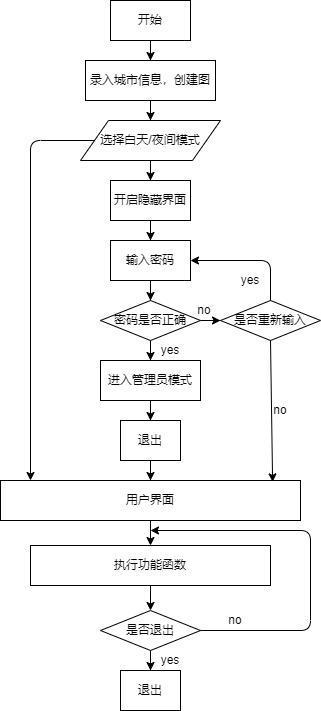
\includegraphics[width=\linewidth]{主函数.png}
\caption{主函数流程图}
\end{figure}

\section{详细设计}
\subsection{定义}	
\begin{figure}[H] 
\centering
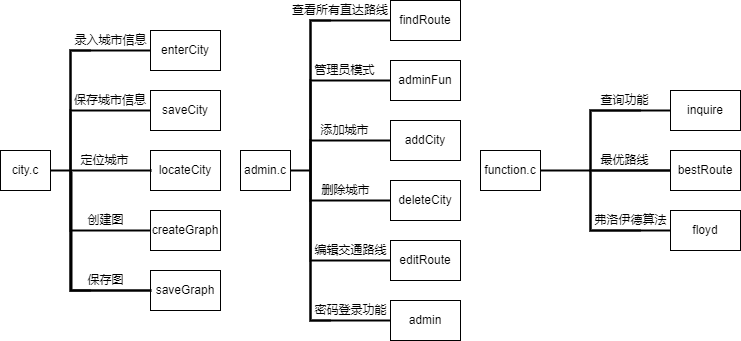
\includegraphics[width=250pt]{结构库.png}
\caption{结构库}	
\end{figure}
\begin{figure}[H] 
\centering
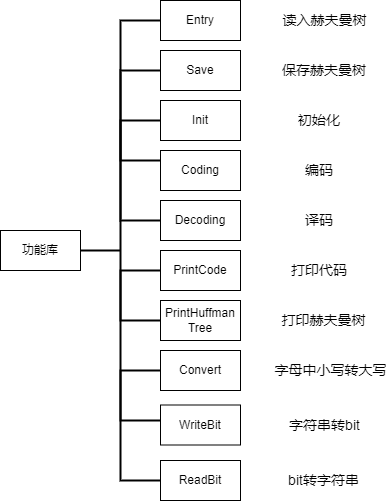
\includegraphics[width=250pt]{功能库.png}
\caption{功能库}	
\end{figure}
\lstinputlisting[language=C]{./code/definition.h}
\subsection{重要函数}
\subsubsection{字符串转比特流}
\begin{lstlisting}[language=c,caption={WriteBit}]
Status WriteBit(char code[])//将字符串转化为bit:开头4个字节保存了该文件存储的位数,后面的字节为存储内容
{
    char *p;
    int i,j=-1,count,num,left;
    printf("请输入代码存储文件名:");
    fflush(stdin);gets(name);strcat(name,".txt");
    fp=fopen(name,"wb");
    count=strlen(code);//字符串个数
    num=count/8;//存储字符需要的字节数
    left=count%8;//字符串剩余不足8位的个数
    if(left==0)
    {
        p=(char*)malloc(sizeof(char)*num);
        memset(p,0,num);
    }
    else
    {
        p=(char*)malloc(sizeof(char)*(num+1));
        memset(p,0,num+1);
    }
    for(i=0;i<count;i++)//位运算,每8个字符以2进制的形式储存在一个字符中
    {
        if(i%8==0) j++;
        p[j]<<=1;
        code[i]-='0';
        p[j]|=code[i];
    }
    if(left!=0)//如果left不为0,需要把剩余的几个位向左边靠拢
    {
        p[j]<<=8-left;
        fwrite(&count,sizeof(count),1,fp);
        fwrite(p,1,num+1,fp);
    }
    else
    {
        fwrite(&count,sizeof(count),1,fp);
        fwrite(p,1,num,fp);
    }
    fclose(fp);
}
\end{lstlisting}
\subsubsection{比特流转字符串}
\begin{lstlisting}[language=c,caption={ReadBit}]
Status ReadBit()//bit转字符串
{
    strcpy(huffmanCode,"");
    char *p;
    int i,j=-1,count,num,left,t=0;
    unsigned char flag=128; //即0b1000000,用于做位运算,注意要用无符号的字符型
    printf("请输入代码存储文件名:");
    fflush(stdin);gets(name);strcat(name,".txt");
    if((fp=fopen(name,"rb"))==NULL)
    {
        printf("该文件夹下无%s!\n",name);
        return ERROR;
    }
    fread(&count,sizeof(count),1,fp);
    num=count/8;
    left=count%8;
    if(left==0)
    {
        p=(char*)malloc(sizeof(char)*num);
        fread(p,1,num,fp);
    }
    else
    {
        p=(char*)malloc(sizeof(char)*(num+1));
        fread(p,1,num+1,fp);
    }
    fclose(fp);
    for(i=0;i<count;i++)
    {
        if(i%8==0)
        {
            j++;
            flag=128;
        }
        if((p[j]&flag)) huffmanCode[t]='1';
        else huffmanCode[t]='0';
        t++;
        flag/=2;
    }
    return OK;
}
\end{lstlisting}

\section{用户手册}
\subsection{界面}
\begin{figure}[H] 
\centering
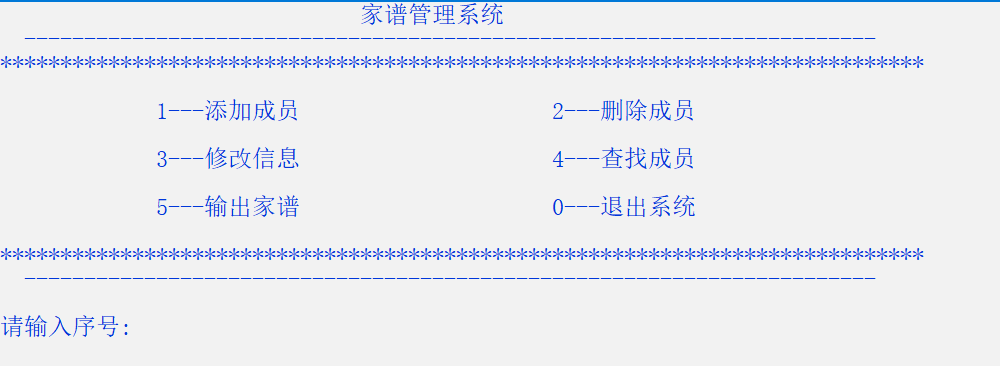
\includegraphics[width=\linewidth]{界面.png}
\caption{用户界面}
\end{figure}
\lstinputlisting[caption={hfmTree.txt}]{./txt/hfmTree.txt}
\subsection{初始化}
在原有树的基础上进行修改和添加字符集操作。
\begin{figure}[H] 
\centering
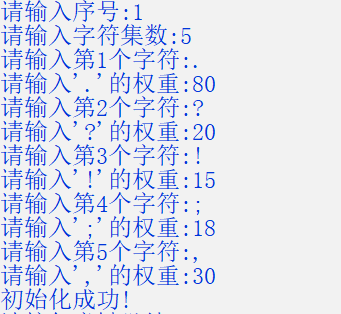
\includegraphics[width=200pt]{初始化.png}
\caption{初始化字符集}	
\end{figure}
\begin{figure}[H] 
\centering

\includegraphics[width=\linewidth]{初始化保存.png}
\caption{保存新的赫夫曼树}	
\end{figure}
\lstinputlisting[caption={Tree1.txt}]{./txt/Tree1.txt}
\subsection{编码}
\begin{figure}[H] 
\centering
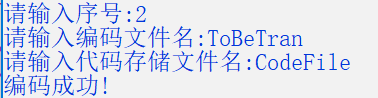
\includegraphics[width=\linewidth]{编码.png}
\caption{编码}	
\end{figure}
\lstinputlisting[caption={ToBeTran.txt}]{./txt/ToBeTran.txt}
CodeFile仅占19字节。
\begin{figure}[H] 
\centering
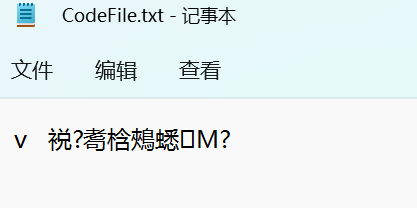
\includegraphics[width=\linewidth]{代码.png}
\caption{代码}	
\end{figure}
\subsection{译码}
\begin{figure}[H] 
\centering
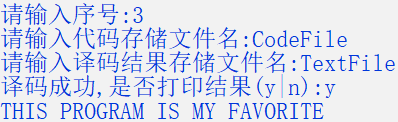
\includegraphics[width=\linewidth]{译码.png}
\caption{译码}	
\end{figure}
\lstinputlisting[caption={TextFile.txt}]{./txt/TextFile.txt}
\subsection{打印代码文件}
\begin{figure}[H] 
\centering
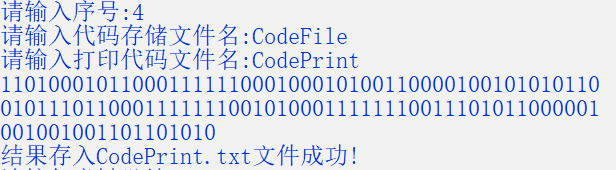
\includegraphics[width=\linewidth]{打印代码.png}
\caption{打印代码文件}	
\end{figure}
未进行压缩的代码占122字节(包含换行符)。
\lstinputlisting[caption={CodePrint.txt}]{./txt/CodePrint.txt}
\subsection{打印赫夫曼树}
\begin{figure}[H] 
\centering
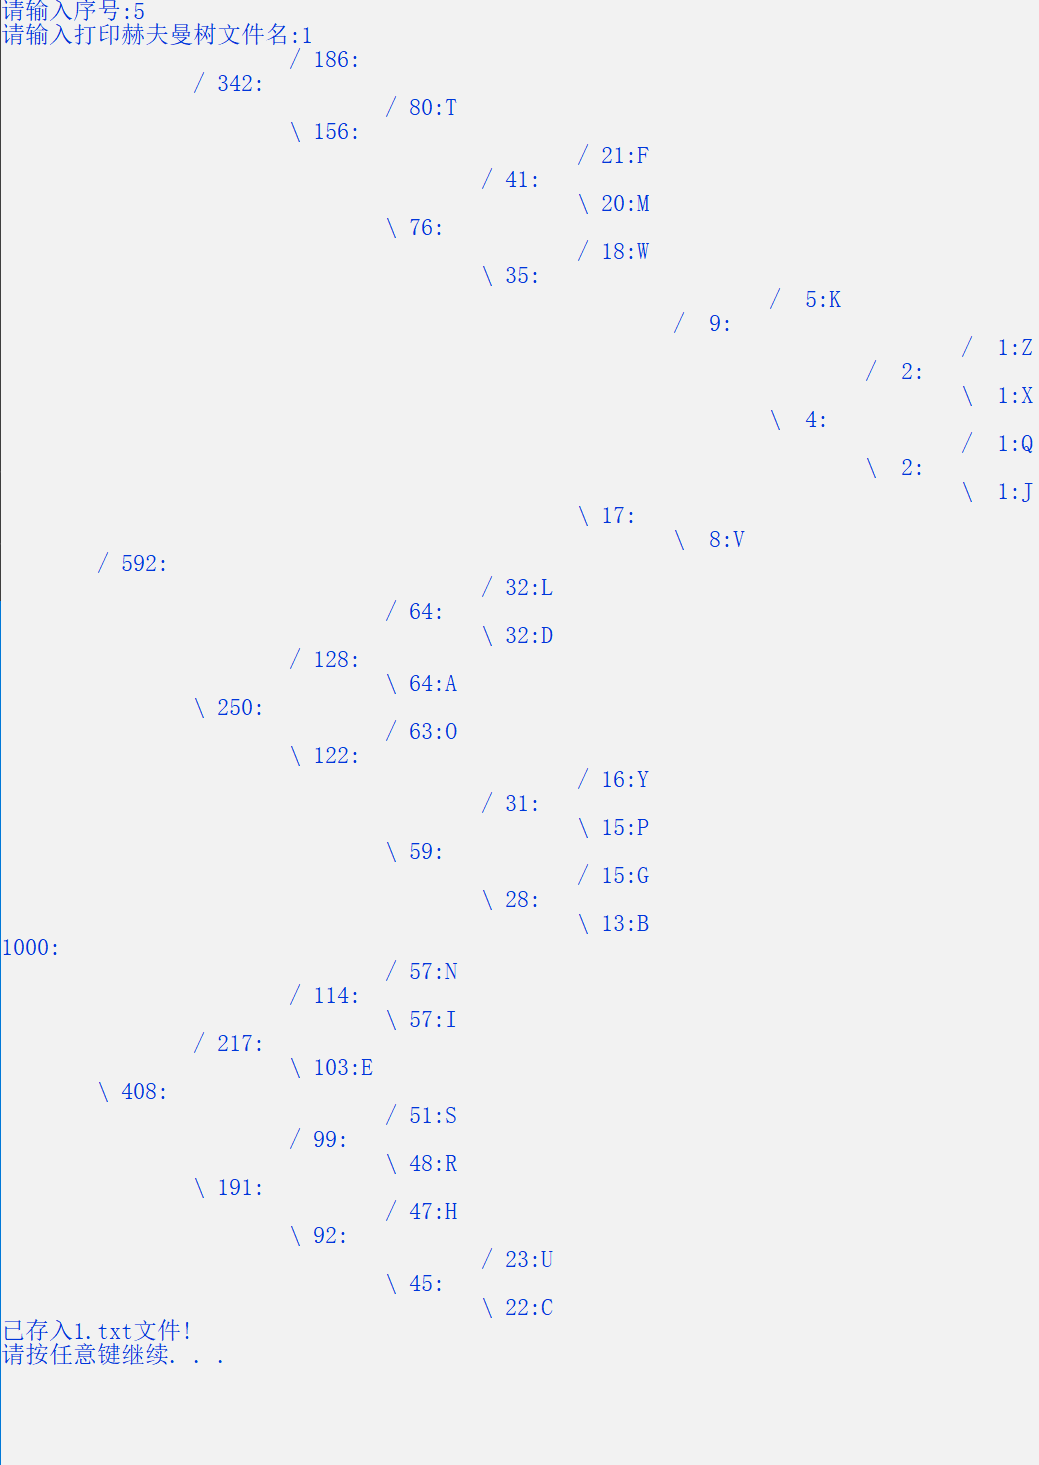
\includegraphics[width=\linewidth]{打印树.png}
\caption{打印赫夫曼树}	
\end{figure}
\begin{figure}[H] 
\centering
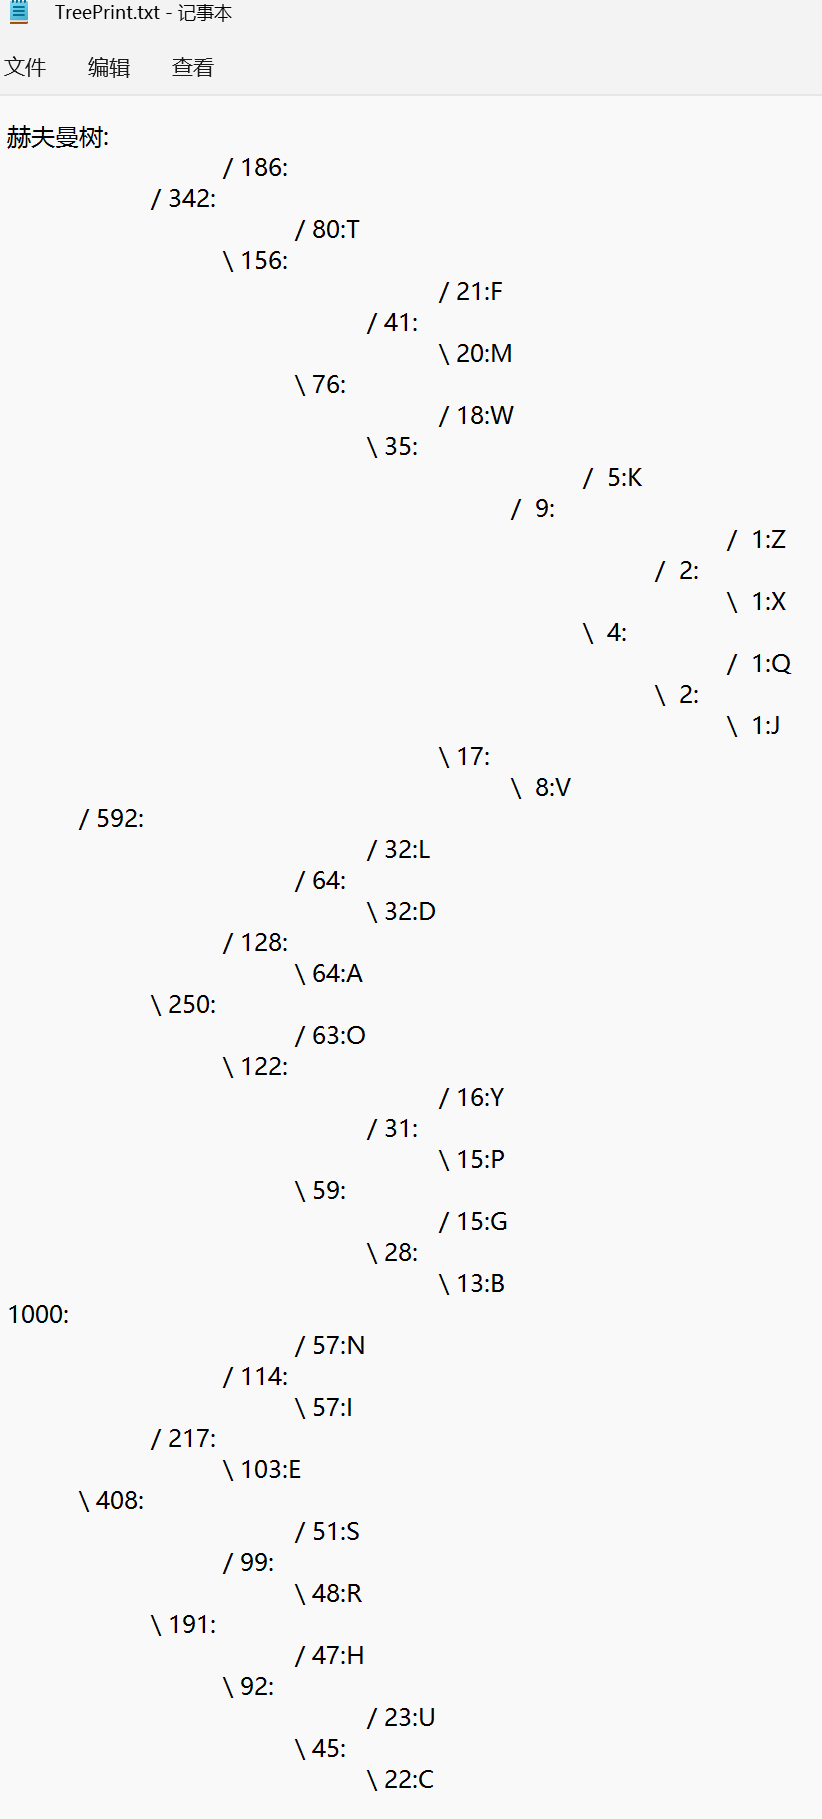
\includegraphics[width=300pt]{树.png}
\caption{TreePrint.txt}	
\end{figure}

\section{心得体会}
这次课程设计的心得体会通过实践我们的收获如下:\par
1.在这次的赫夫曼编码译码的过程中,我们更深刻地了解了赫夫曼树的特点与用法。\par
2.在做一个较大的程序过程中,应该学会边编写程序边运行,即完成了一个功能,也要对其调试,这样有利于我们高效地完成项目,并在调试BUG的过程可以大大减小难度。\par
3.必须要有良好的编程习惯。首先编码风格要统一规范,这样不仅有利于代码的阅读,更有利于代码的维护。其次在一些代码方面要细心谨慎,减少BUG出现的机率。\par
4.更加系统地学习了C语言的二进制位操作,对文件函数的运用更加熟练。

\newpage 
\section{附录}
\subsection{definition.h}
\lstinputlisting[language=C]{./code/definition.h}
\subsection{main.c}
\lstinputlisting[language=C]{./code/main.c}
\subsection{huffman.c}
\lstinputlisting[language=C]{./code/huffman.c}
\subsection{function.c}
\lstinputlisting[language=C]{./code/function.c}

\end{document}
